\subsubsection{Upload}
\label{sec:view_upload}

\paragraph{}
The upload page (figure \ref{fig:upload_view}) allows the user to upload new files and to manage the contents of their upload directory. It is linked to under the session tab of the default ROME navigation bar. Files in the upload directory are simply raw data for parsing and are not integrated into ROME in any way and can be deleted at will. Multiple files may be uploaded as an archive (zip, tar, bzip) and will automatically be unpacked into the user's upload directory. The list of uploaded files is presented as a directory tree and can be updated via an ajax call should the contents change without a page reload. 

\paragraph{}
Although only registered users are able to uploaded files, the unpacking of archives could pose a security risk if ROME is accessible via the internet. If this is a major concern, or if file sizes are likely to be too large to reasonably transfer over http, there is no reason why the users should not be given scponly (\url{http://sublimation.org/scponly}) accounts providing chrooted sftp access to their upload directory. 


\begin{figure}[h]
\centering
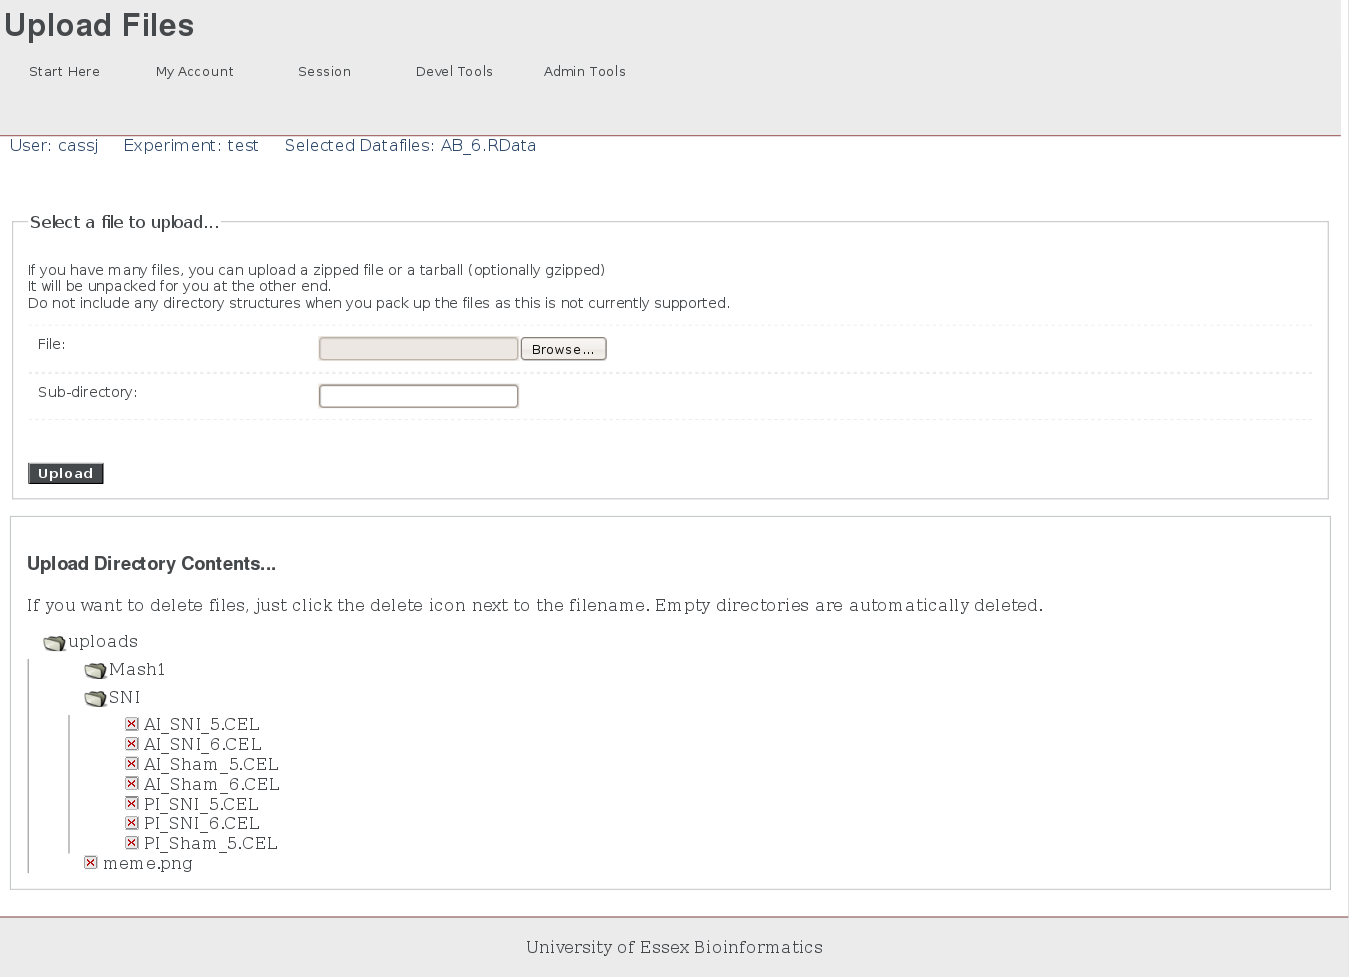
\includegraphics[scale=0.45, angle=90]{../rome/docs/images/screenshots/upload}
\caption{The Upload Page}\label{fig:upload_view}
\end{figure}

\clearpage
